\documentclass{beamer}
\usetheme{Boadilla}
\usepackage[utf8]{inputenc}
\usepackage[czech]{babel}
\usepackage{datetime}
\newdate{date}{05}{05}{2022}
\title{Kalibrace a monitorování astročásticových teleskopů}
\author{Daniel Staník}
\institute{
SLO}
\date{\displaydate{date}}

\setbeamertemplate{background} {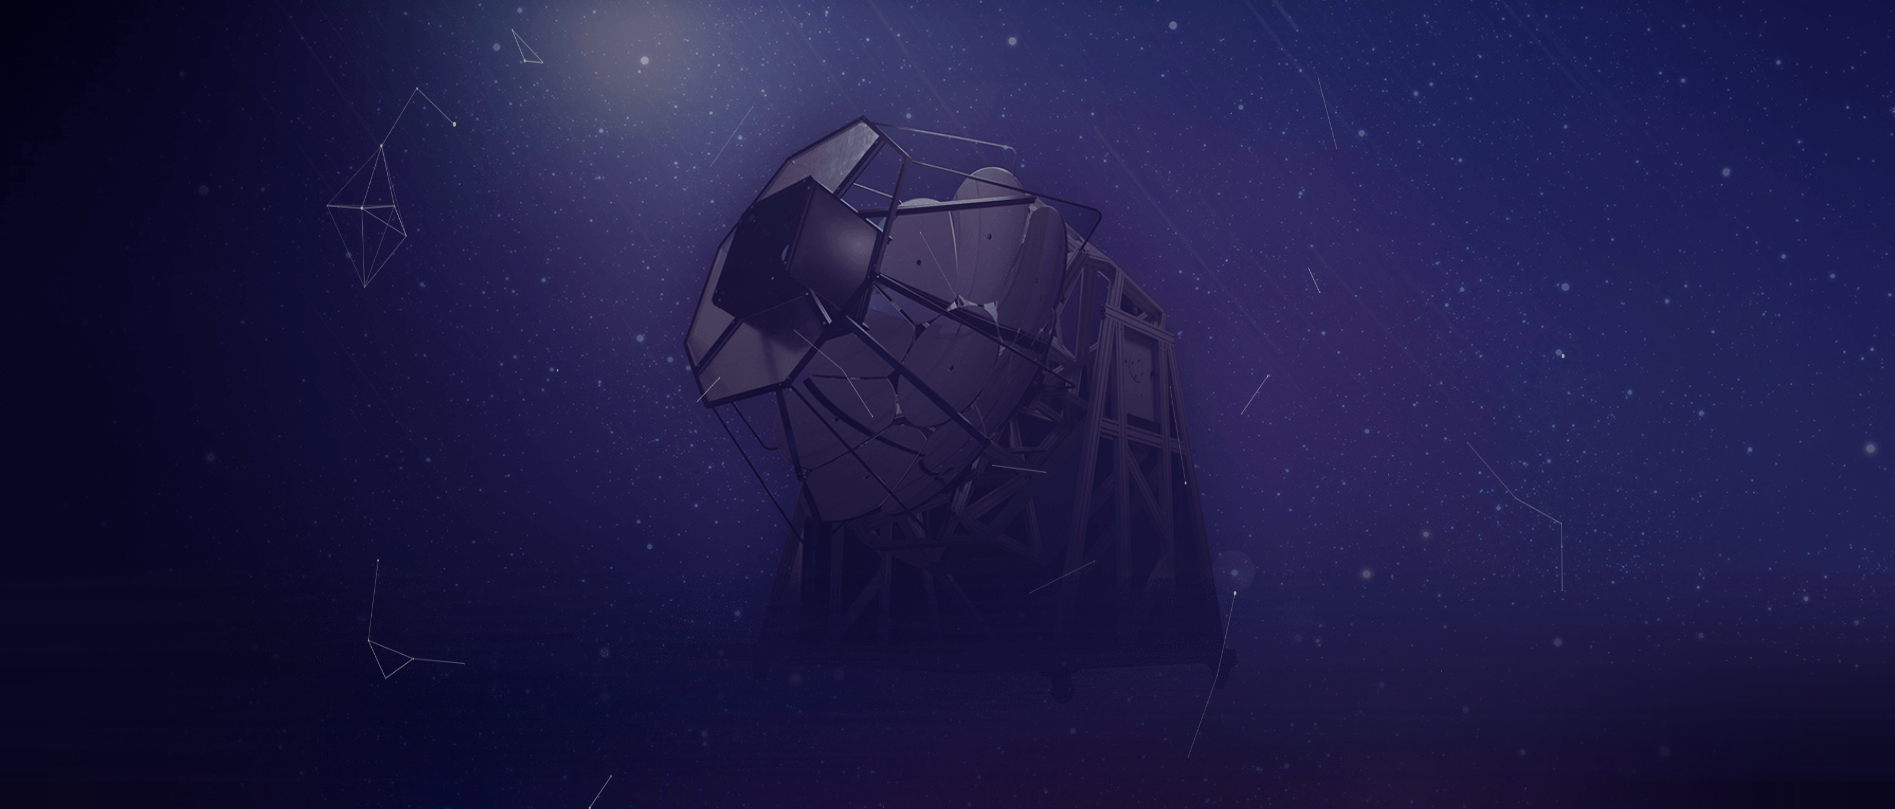
\includegraphics[width=550 pt,height=\paperheight]{fast.png}}





\setbeamercolor{author}{fg=green} 
\setbeamercolor{institute}{fg=green} 
\setbeamercolor{date}{fg=green}
%\setbeamercolor{frametitle}{fg=yellow}

%\setbeamercolor{caption name}{fg=yellow}







\makeatletter
\setbeamertemplate{footline}
{%
  \leavevmode%
  \hbox{%
  \begin{beamercolorbox}[wd=.333333\paperwidth,ht=2.25ex,dp=1ex,center]{author in head/foot}%
    \usebeamerfont{author in head/foot}%
    \insertshortauthor\expandafter\ifblank\expandafter{\beamer@shortinstitute}{}
    {~~(\insertshortinstitute)}
  \end{beamercolorbox}%
  \begin{beamercolorbox}[wd=.333333\paperwidth,ht=2.25ex,dp=1ex,center]{title in head/foot}%
%    \usebeamerfont{title in head/foot}\insertshorttitle
  \end{beamercolorbox}%
  \begin{beamercolorbox}[wd=.333333\paperwidth,ht=2.25ex,dp=1ex,right]{date in head/foot}%
    \usebeamerfont{date in head/foot}\insertshortdate{}\hspace*{2em}
    \usebeamercolor[fg]{page number in head/foot}%
    \usebeamerfont{page number in head/foot}%
    \usebeamertemplate{page number in head/foot}\hspace*{2ex} 
  \end{beamercolorbox}}%
  \vskip0pt%
}
\makeatother












\begin{document}


\begin{frame}

{
\setbeamercolor{title}{fg=yellow}
\setbeamercolor{normal text}{fg=green}
\titlepage
}
\end{frame}


\setbeamertemplate{background}{}
%\setbeamercolor{title}{fg=blue}
%\setbeamercolor{frametitle}{fg=blue}
%\setbeamercolor{normal text}{fg=black}
%\setbeamercolor{caption name}{fg=blue}

\begin{frame}
\frametitle{Cíle práce}
\begin{itemize}
 \item Dlouhodobě otestovat stávající světelný UV zdroj pro kalibraci fluorescenčního teleskopu FAST. 
 \item Navrhnout a pokusit se realizovat případná vylepšení stability. 
 \item Provést měření vlastností optoelektronických prvků vhodných pro účely stabilizačního zdroje.
 \item Analýza kalibračních dat z teleskopu FAST získaných za pomoci osvěcování UV zdrojem.
\end{itemize}

\end{frame}



%\begin{frame}
%\frametitle{Obsah}
%\begin{itemize}
% \item FAST - fluorescenční detektor vysokoenergetických kosmických částic (UHECR).  
% \item Testování pulzního UV kalibračního zdroje.
% \item Úpravy pulzního UV kalibračního zdroje.
% \item Analýza kalibračních dat.
%\end{itemize}

%\end{frame}






\begin{frame}
\frametitle{Teleskop FAST}
\begin{itemize}
 \item Fluorescenční teleskop pro detekci kosmických částic s extrémní energií (UHECR) ($10^{18}$ až $10^{20}$ eV).
 \item Fluorescenční technika detekce - detekce deexcitačního slabého UV spektra dusíkových molekul atmosféry.
 \item Detekční část - čtyři fotonásobiče a superodrazná UV zrcadla.
 \item Dnes v provozu 4 prototypy.
 \item Budoucí účel - osazení velké plochy teleskopy tohoto typu a rekonstrukce spršek vyvolaných UHECR částicemi.
\end{itemize}

\end{frame}

\begin{frame}
\frametitle{Teleskop FAST}
\begin{columns}[t]
\column{.5\textwidth}
\centering
\begin{figure}[H]
\includegraphics[scale=0.3, angle = 0, origin = c]{../BachelorThesis/pictures/fastTheoretical.png}\\
\caption{Návrh teleskopu.}
\end{figure}
\column{.5\textwidth}
\centering
\begin{figure}[H]
\includegraphics[scale=0.09, angle = 0, origin = c]{../BachelorThesis/pictures/FASTReal}\\
\caption{Teleskop FAST.}
\end{figure}
\end{columns}



\end{frame}



\begin{frame}
\frametitle{Vývoj a testování kalibračního UV zdroje}
\begin{itemize}
 \item Nutnost kalibrace teleskopu jako optické soustavy. Detekční části díky různým vlivům podléhají degradaci.
 \item K tomu účelu - pulzní kalibrační UV zdroj založen na diodách. Netestován, nutnost ověření jeho funkčnosti a návrh případných úprav či jiných konceptů. Proto sestavena aparatura pro dlouhodobé měření stability zdroje.
 \item Nutno ověřit dva parametry - stabilita výkonu a stabilita geometrie pulzů. Měření prováděno v intervalu dvou týdnů. K měření výkonu užit PM16 měřicí přístroj optického výkonu a k měření pulzní geometrie - fotonásobič + osciloskop.
\end{itemize}





\end{frame}

\begin{frame}
%\frametitle{Teleskop FAST}


 \begin{figure}[H]
 \centering
 \includegraphics[scale=0.07, angle = 0, origin = c]{../BachelorThesis/pictures/KarlsRuhe}
 \caption{Prototyp kalibračního zdroje.}
 \label{UVsource}
\end{figure}


\end{frame}





\begin{frame}
%\frametitle{Teleskop FAST}




 \begin{figure}[H]
 \centering
 \includegraphics[scale=0.07, angle = 0, origin = c]{../BachelorThesis/pictures/aprature1b}
 \caption{Testovací aparatura.}
 \label{UVsource}
\end{figure}


\end{frame}

\begin{frame}
\frametitle{Výsledky měření}
\begin{columns}[t]
\column{.5\textwidth}
\centering
\begin{figure}[H]
\includegraphics[width=6.5cm,height=4cm]{../BachelorThesis/pictures/powers}\\
\caption{Vývoj výkonu.}
\end{figure}
\column{.5\textwidth}
\centering
\begin{figure}[H]
\includegraphics[width=6.5cm,height=4cm]{../BachelorThesis/pictures/Height}\\
\caption{Vývoj výšky pulzu.}
\end{figure}
\end{columns}



\end{frame}



\begin{frame}
\frametitle{Výsledky měření}
\begin{columns}[t]
\column{.5\textwidth}
\centering
\begin{figure}[H]
\includegraphics[width=6.5cm,height=4cm]{../BachelorThesis/pictures/rise}\\
\caption{Vývoj doby náběhu.}
\end{figure}
\column{.5\textwidth}
\centering
\begin{figure}[H]
\includegraphics[width=6.5cm,height=4cm]{../BachelorThesis/pictures/Slope}
\caption{Vývoj sklonu náběžné hrany.}
\end{figure}
\end{columns}



\end{frame}




\begin{frame}
\frametitle{Výsledky měření}
\begin{itemize}
 \item Nalezen zásadní problém - výrazný rostoucí trend ve výkonu. Potvrzeno fotonásobičem i PM16. Pulzní geometrie - doba náběhu a sklon nemají dlouhodobý trend.
 \item Hlavní příčinnou jsou degradační procesy v samotných diodách. Viz další stránka se samotným chováním diody.
 \item Možná oprava - přidaní zpětnovazební UV detekční diody, podle které se bude upravovat proud LEDkou. 

\end{itemize}


\end{frame}



\begin{frame}
\frametitle{Degradace osamocené LED diody.}
 \begin{figure}[H]
 \centering
 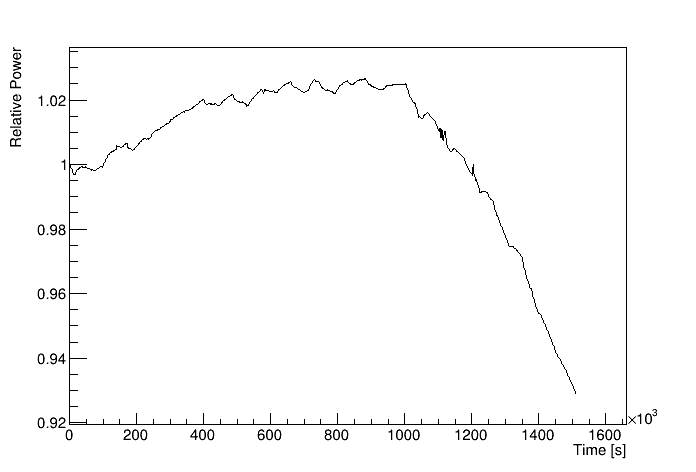
\includegraphics[scale=0.4, angle = 0, origin = c]{corrected1}
 \caption{Degradace osamocené LED diody.}
 \label{UVsource}
\end{figure}


\end{frame}



\begin{frame}
\frametitle{Optická zpětná vazba}


\begin{itemize}
 \item Nastavování výkonu podle detekované hodnoty - detekce výšky pulzů za pomoci fotodiody.
 \item Nutnost změření fotodiody - závislosti chování na teplotě, odezvy na pulzy a dlouhodobé stability.


\end{itemize}


 \begin{figure}[H]
 \centering
 \includegraphics[scale=0.045, angle = 0, origin = c]{../BachelorThesis/pictures/optomechanics.png}
 \caption{Zpětnovazební optomechanika.}
 \label{UVsource}
\end{figure}


\end{frame}


\begin{frame}

 \begin{figure}[H]
 \centering
 \includegraphics[scale=0.4, angle = 0, origin = c]{../BachelorThesis/pictures/1V}
 \caption{Závislost temných proudů na teplotě.}
 \label{UVsource}
\end{figure}


\end{frame}

\begin{frame}

 \begin{figure}[H]
 \centering
 \includegraphics[scale=0.4, angle = 0, origin = c]{../BachelorThesis/pictures/pulse.png}
 \caption{Detekovaný pulz přes I/U převodník.}
 \label{UVsource}
\end{figure}


\end{frame}






\begin{frame}

 \begin{figure}[H]
 \centering
 \includegraphics[scale=0.4, angle = 0, origin = c]{../BachelorThesis/pictures/ArtiAging.png}
 \caption{Stárnutí detekční fotodiody.}
 \label{UVsource}
\end{figure}


\end{frame}



\begin{frame}

\begin{itemize}
 \item 
 Použití desky Nucleo F446RE. Nastavení synchronního vzorkování za pomoci provázání interních časovačů.
 \item 
 Navzorkování pulzů, a vyvození výšky pulzu - získání hodnoty aktuálního výkonu. Tato hodnota následně použita do PID regulátoru. 
 
 \end{itemize}
 \begin{figure}[H]
 \centering
 \includegraphics[scale=0.3, angle = 0, origin = c]{../BachelorThesis/pictures/PWMSampling.png}
 \caption{Synchronizované vzorkování.}
 \label{UVsource}
\end{figure}


\end{frame}


\begin{frame}

 \begin{figure}[H]
 \centering
 \includegraphics[scale=0.4, angle = 0, origin = c]{../BachelorThesis/pictures/LongTime.png}
 \caption{Test upraveného zdroje.}
 \label{UVsource}
\end{figure}


\end{frame}



\begin{frame}
\frametitle{Analýza kalibračních dat}
\begin{itemize}

 \item Hlavní účel analýzy - získání relativních odezvových konstant pro 4 fotonásobiče.

 \begin{figure}[H]
 \includegraphics[scale=0.28, angle = 0, origin = c]{../BachelorThesis/pictures/orientation2}\\
\caption{Umístění zdroje.}
 \end{figure}
 
 \end{itemize}
 \end{frame}  
 
\begin{frame}
\frametitle{Nasvícení fotonásobičů}
 \begin{figure}[H]
 \centering
 \includegraphics[scale=0.265, angle = 0, origin = c]{../BachelorThesis/pictures/CalibPulses}
 \caption{Signál viděný fotonásobiči.}
 \label{UVsource}
\end{figure}


\end{frame}  
 
\begin{frame}
\frametitle{Ukázka distribuce}
 \begin{figure}[H]
 \centering
 \includegraphics[scale=0.18, angle = 0, origin = c]{../BachelorThesis/pictures/right}
 \caption{Ukázka fitování distribucí maximální výšky kalibračních pulzů a srovnání pro 4 fotonásobiče.}
 \label{UVsource}
\end{figure}


\end{frame} 


\begin{frame}
\frametitle{Porovnání výsledků se simulacemi}

\begin{table}[H]
\centering
\begin{tabular}{|c|c|c|c|}
\hline
   & pravá & levá & spodek \\ \hline
$c_0$ & $0.2314 \pm 0.0002$    & $1$   				   & $0.1070 \pm 0.0002$     \\ \hline
$c_1$ & $0.1397 \pm 0.0002$    & $0.7485 \pm 0.0003$   & $0.8061 \pm 0.0003$      \\ \hline
$c_2$ & $0.9304 \pm 0.0004$    & $0.2138 \pm 0.0002$   & $0.1631 \pm 0.0002$      \\ \hline
$c_3$ & $1$    				   & $0.2462 \pm 0.0002$   & $1$      \\ \hline
\end{tabular}
\caption{Naměřené odezvové konstanty.}
 \label{CalibConstTbl}
\end{table}






\begin{table}[H]

\begin{tabular}{|c|c|c|c|}
\hline
   & pravá & levá & spodek \\ \hline
$c_0$ & $0.48$    & $0.95$   & $0.44$     \\ \hline
$c_1$ & $0.41$    & $1$   	 & $0.98$      \\ \hline
$c_2$ & $1$    	  & $0.41$   & $0.46$      \\ \hline
$c_3$ & $0.95$    & $0.46$   & $1$      \\ \hline
\end{tabular}
\caption{Konstanty ze simulace.}
 \label{CalibConstTblSim}
\end{table}


\end{frame}


\begin{frame}
\frametitle{Zhodnocení}
\begin{itemize}
 \item Podařilo se otestovat stávájící koncept UV zdroje. Byla zjištěna dlouhodobá změna výkonu, s největší pravděpodobností způsobena procesy v LED diodě.
 \item Jako řešení otestována optická vazba využívající synchronizovaného vzorkování s regulátorem na bázi PID. Bylo dosaženo lepší stability.
 \item Z kalibračních dat se podařilo vyvodit odezvové konstanty pro fotonásobiče, ale neshodují se s teoretickými.
\end{itemize}

\end{frame}


\begin{frame}{}
  \centering \Large
  \emph{Děkuji za pozornost.}
\end{frame}
















\end{document}

